\taskpic{ По наклонной плоскости, образующей угол $\alpha$ с
  горизонтом, скатывается массивный полый цилиндр массы $M$. По
  поверхности цилиндра бежит собака таким образом, что она всё время
  занимает наивысшее положение на поверхности цилиндра. Определите, с
  каким ускорением скатывается цилиндр, если масса собаки $m$. }
{
  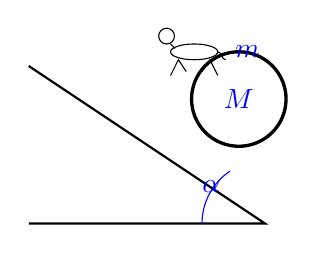
\begin{tikzpicture}
    \coordinate (a) at (0,2);
    \coordinate (b) at (3,0);
    \coordinate (c) at (0,0);
    \draw[thick] (a) -- (b) -- (c);
    \draw[very thick,rotate around={-atan2(3,2):(3,0)}] (1.5,0.6) circle
    (0.6cm) node[blue] {$M$};
    % собака
    \begin{scope}[yshift=1.88cm,xshift=1.8cm]
      \draw (0,0) -- (0.1,0.2) -- (0.2,0.05);
      \draw (0.4,0.05) -- (0.5,0.2) -- (0.6,0);
      \draw (0.3,0.3) ellipse (0.3 and 0.1) node[blue,right=0.4cm] {$m$};
      \draw (-0.05,0.5) circle (0.1cm);
      \draw (0,0.4) -- ++(-45:0.08cm);
      \draw (0.6,0.3) to[out=0,in=180] (0.7,0.2);
    \end{scope}
    % угол
    \draw[blue] (2.2,0) arc (180:180-atan2(3,2):0.8cm) node[below left]
    {$\alpha$};  
  \end{tikzpicture}
}
% Сивухин
